\documentclass[10pt, aspectratio=169]{beamer}

% --- Cấu hình Tiếng Việt và Font ---
\usepackage{fontspec}
% \usepackage[utf8]{inputenc}
% \usepackage[T5]{fontenc}
% \usepackage[vietnam]{babel}
% \usepackage{helvet} % Font sans-serif dễ đọc cho slide

% --- Các gói hỗ trợ ---
\usepackage{amsmath, amsfonts, amssymb} % Toán học
\usepackage{booktabs} % Kẻ bảng đẹp
\usepackage{graphicx} % Chèn ảnh
\usepackage{tikz} % Vẽ sơ đồ
\usetikzlibrary{shapes, arrows, positioning}
\usepackage{listings} % Chèn code (nếu cần)
\usepackage{caption}
\usepackage{array}
\usepackage{makecell}
\setcellgapes{2pt}

% --- Theme và Màu sắc ---
\usetheme{Frankfurt}
\usecolortheme{crane}
% Tùy chỉnh footer cho gọn
\setbeamertemplate{navigation symbols}{}
\setbeamertemplate{footline}[frame number]

\AtBeginSection[]
{
  \begin{frame}[plain, noframenumbering]
  \frametitle{Contents}
  \tableofcontents[currentsection, hideallsubsections]
  \end{frame}
}

% --- Thông tin bài báo cáo ---
\title[Data Preparation - NLP Project]{Project Overview}
\subtitle{Topic: Neurosymbolic Reasoning}
\author{Nguyễn Ngọc Cảnh, Huỳnh Gia Bảo, Nguyễn Đức Trí,\\Phan Huỳnh Minh Khôi, Trần Lý Nhật Hào}
\institute{Faculty of Information Technology\\University of Science - VNUHCM}
\date{January 30, 2026}

\begin{document}

% Slide 1: Title
\begin{frame}[plain, noframenumbering]
  \titlepage
\end{frame}

% Slide 2: Mục lục
\begin{frame}[plain, noframenumbering]{Contents}
  \tableofcontents
\end{frame}

% --- PART 1: MOTIVATION ---
\section{Motivation for Neurosymbolic AI}

\begin{frame}{Classical AI: Rule-based/Symbolic AI}
  \begin{columns}[T] % Tùy chọn [T] để căn lề trên cùng cho cả 2 cột
    % --- CỘT TRÁI ---
    \begin{column}{0.48\textwidth}
      \centering
      \begin{block}{\textbf{Knowledge Base}}
        $\forall x: \text{Human}(x) \rightarrow \text{Wibu}(x)$ \\
        \hfill {\footnotesize (All humans are wibu.)} \\
        $\text{Human}(\text{Huy})$ \\
        \hfill {\footnotesize (Huy is human.)}
      \end{block}
      \pause
      \begin{block}{\textbf{Deduction Mechanism}}
        \begin{tabular}{l}
          $A \rightarrow B$ \\
          $A$ \\
          \midrule
          \hfill $\therefore B$
        \end{tabular}
        \hfill {\footnotesize (Syllogism/Modus ponens)}
      \end{block}
      \pause
      \begin{block}{\textbf{Conclusion}}
        $\text{Wibu}(\text{Huy})$ \\
        \hfill {\footnotesize (Huy is wibu.)}
      \end{block}
    \end{column}
    % --- CỘT PHẢI ---
    \begin{column}{0.48\textwidth}
      \pause
      \begin{exampleblock}{\textbf{Pros}}
        \begin{itemize}
          \item Explainability
          \item Data Efficiency
          \item Abstract Reasoning
        \end{itemize}
      \end{exampleblock}
      % \vspace{0.3cm}
      \pause
      \begin{alertblock}{\textbf{Cons}}
        \begin{itemize}
          \item Brittleness
          \item Scalability
          \item Poor Perception
        \end{itemize}
      \end{alertblock}
      \vspace{0.3cm}
      \pause
      $\boldsymbol{\Rightarrow}$ \textbf{reliable but inflexible.}
    \end{column}
  \end{columns}
\end{frame}

\begin{frame}{Modern AI: Data-driven/Neural Networks}
  \begin{columns}[T] % Tùy chọn [T] để căn lề trên cùng cho cả 2 cột
    % --- CỘT TRÁI ---
    \begin{column}{0.48\textwidth}
      \centering
      \begin{block}{\textbf{Neural Networks}}
        \centering
        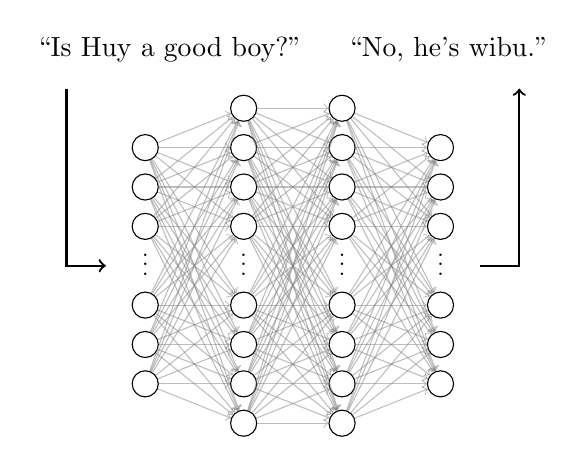
\begin{tikzpicture}[scale=0.5]
          % --- NEURAL NETWORK ---
          \foreach \i\shift in {1/-3, 2/-2, 3/-1, 4/1, 5/2, 6/3} {
            \node[circle, draw, minimum size=0.25cm] (fc1\i) at (0, \shift) {};
          }
          \node[scale=5/6, circle, minimum size=0.25cm] (fc1...) at (0, 0.2) {$\vdots$};

          \foreach \i\shift in {1/-4, 2/-3, 3/-2, 4/-1, 5/1, 6/2, 7/3, 8/4} {
            \node[circle, draw, minimum size=0.25cm] (fc2\i) at (2.5, \shift) {};
          }
          \node[scale=5/6, circle, minimum size=0.25cm] (fc2...) at (2.5, 0.2) {$\vdots$};

          \foreach \i\shift in {1/-4, 2/-3, 3/-2, 4/-1, 5/1, 6/2, 7/3, 8/4} {
            \node[circle, draw, minimum size=0.25cm] (fc3\i) at (5, \shift) {};
          }
          \node[scale=5/6, circle, minimum size=0.25cm] (fc3...) at (5, 0.2) {$\vdots$};

          \foreach \i\shift in {1/-3, 2/-2, 3/-1, 4/1, 5/2, 6/3} {
            \node[circle, draw, minimum size=0.25cm] (fc4\i) at (7.5, \shift) {};
          }
          \node[scale=5/6, circle, minimum size=0.25cm] (fc4...) at (7.5, 0.2) {$\vdots$};

          \foreach \i in {1,...,8} {
            \foreach \j in {1,...,6} {
              \draw[->, gray, opacity=0.5] (fc1\j) -- (fc2\i);
              \draw[->, gray, opacity=0.5] (fc3\i) -- (fc4\j);
            }
            \foreach \k in {1,...,8} {
              \draw[->, gray, opacity=0.5] (fc2\i) -- (fc3\k);
            }
          }

          \visible<2->{
            % --- INPUT ---
            \draw[->, thick] (-2, 4.5) -- (-2, 0) -> (-1, 0);
            \node[right] at (-3, 5.5) {``Is Huy a good boy?''};
          }

          \visible<3->{
            % --- OUTPUT ---
            \draw[->, thick] (8.5, 0) -- (9.5, 0) -> (9.5, 4.5);
            \node[left] at (10.5, 5.5) {``No, he's wibu.''};
          }
        \end{tikzpicture}
      \end{block}
    \end{column}
    % --- CỘT PHẢI ---
    \begin{column}{0.48\textwidth}
      \visible<4->{
        \begin{exampleblock}{\textbf{Pros}}
          \begin{itemize}
            \item Generalization \& Robustness
            \item Perception
            \item Automated Feature Extraction
          \end{itemize}
        \end{exampleblock}
      }
      \visible<5->{
        \begin{alertblock}{\textbf{Cons}}
          \begin{itemize}
            \item Lack of Explainability
            \item Data \& Resource Hungry
            \item Hallucination
          \end{itemize}
        \end{alertblock}
      }
      \vspace{0.3cm}
      \visible<6->{
        $\boldsymbol{\Rightarrow}$ \textbf{flexible but unreliable.}
      }
    \end{column}
  \end{columns}
\end{frame}

\begin{frame}{Neurosymbolic AI: A Hybrid Approach}
  \begin{columns}
    \begin{column}{0.28\textwidth}
      \begin{figure}
        
\includegraphics[width=\linewidth]{imgs/Thinking fast and slow.jpg}
      \end{figure}
    \end{column}

    \begin{column}{0.7\textwidth}
      \centering
      
\begin{tikzpicture}
        \visible<1-6>{
          \node[scale=0.8] at (0, 0) {\textbf{SYSTEM 1 (FAST)}};
          \node[scale=0.8] at (0, -0.4) {\footnotesize Intuition \& Instinct};
          \node[scale=0.8] at (3.55, 0) {\textbf{SYSTEM 2 (SLOW)}};
          \node[scale=0.8] at (3.55, -0.4) {\footnotesize Rational thinking};
        }
        \visible<2-6>{
          \node[rotate=90] at (0, -1.1) {\textbf{=}};
          \node[scale=0.8] at (0, -2) {\textbf{NEURAL NETWORK}};
        }
        \visible<3-6>{
          \node[rotate=90] at (3.55, -1.1) {\textbf{=}};
          \node[scale=0.8] at (3.55, -2) {\textbf{SYMBOLIC ENGINE}};
        }
        \visible<4-6>{
          \node at (1.775, -0.2) {\textbf{+}};
          \node at (5.3, -0.2) {\textbf{=}};
          \node[scale=0.8] at (7.1, 0) {\textbf{HUMAN}};
          \node[scale=0.8] at (7.1, -0.4) {\textbf{INTELLIGENGE}};
        }
        \visible<5-6>{
          \node at (1.775, -2) {\textbf{+}};
          \node at (5.3, -2) {\textbf{=}};
          \node[scale=0.8] at (7.1, -2) {\textbf{NEUROSYMBOLIC AI}};
        }
        \visible<6>{
          \node[rotate=90] at (7.1, -1.1) {\textbf{=}};
        }
        \visible<7->{
          \node[draw, circle, thick, minimum size=0.55cm] (plus) at (1.775, -2) {};
          \node[scale=0.8] at (0, -2) {\textbf{NEURAL NETWORK}};
          \node at (1.775, -2) {\textbf{+}};
          \node[scale=0.8] at (3.55, -2) {\textbf{SYMBOLIC ENGINE}};
          \node at (5.3, -2) {\textbf{=}};
          \node[scale=0.8] at (7.1, -2) {\textbf{NEUROSYMBOLIC AI}};
        }
        \visible<8>{
          \node[draw, thick,
                rounded corners,
                inner sep=6pt] (NFLT) at (1.775, -0.2) {\textbf{Semantic Parsing/Language Formalization}};
          \draw[->, thick] (plus) -- (NFLT);
        }
      \end{tikzpicture}
    \end{column}
  \end{columns}
\end{frame}

\section{Problem Statement}

\begin{frame}{Problem Statement}

    % Part 1: Definition
    \begin{block}{\textbf{Language Formalization}}
        The goal is to learn a mapping function $f: \mathcal{X} \rightarrow \mathcal{Y}$ that translates Natural Language sentences ($x_\text{NL}$) into machine-verifiable First-Order Logic formulas ($y_\text{FOL}$).
    \end{block}
    \pause
    \vspace{0.5cm}

    % Part 2: Visualization Input -> Output
    \begin{columns}[c]

        % Input Column
        \begin{column}{0.35\textwidth}
            \centering
            \textbf{\textcolor{blue}{Input ($x_\text{NL}$)}} \\
            \vspace{0.1cm}
            \scriptsize{\textit{Natural Language}} \\
            \scriptsize{\textit{(Unstructured)}}
            % \vspace{0.1cm}
            \begin{alertblock}{}
                \centering
                \small
                "Every student takes a course."
            \end{alertblock}
        \end{column}

        % Arrow
        \begin{column}{0.11\textwidth}
            % \centering
            \vspace{0.4cm}
            \Huge $\xrightarrow{f(\cdot)}$
        \end{column}

        % Output Column
        \begin{column}{0.45\textwidth}
            \centering
            \textbf{\textcolor{green!40!black}{Output ($y_\text{FOL}$)}} \\
            \vspace{0.1cm}
            \scriptsize{\textit{First-Order Logic}} \\
            \scriptsize{\textit{(Structured)}}
            % \vspace{0.1cm}
            \begin{exampleblock}{}
                \centering
                \footnotesize
                $\forall x (\text{Student}(x) \rightarrow \exists y (\text{Course}(y) \wedge \text{Takes}(x, y)))$
            \end{exampleblock}
        \end{column}

    \end{columns}

    \pause
    \vspace{0.6cm}

    % Part 3: Challenges
    \textbf{Core Challenges:}
    \begin{itemize}
        \item \textbf{The Requirement for Absolute Precision:} Formal languages are syntactically fragile. A formal expression must be 100\% correct to be machine-verifiable.
        \item \textbf{Data Scarcity and the Expert-Data Bottleneck:} Creating NL-FOL pairs requires professionals with deep knowledge of both the domain and the formal syntax.
    \end{itemize}

\end{frame}

\section{Data}
\begin{frame}{Data Source}
\only<1>{
  The data used consists of the \textbf{training sets} of the datasets listed in the table below.
    \begin{table}
      \centering
      \begin{tabular}{@{}llp{8.75cm}@{}}
        \toprule
        \textbf{Source} & \textbf{Volume} & \textbf{Description} \\
        \midrule
        FOLIO & \hfill 1,000 samples & \textbf{With FOL label}, with true/false/uncertain label. \\
        ProofWriter & \hfill 41,400 samples & \textbf{Without FOL label}, with true/false label, with proof. \\
        RuleTaker & \hfill 480,000 samples & \textbf{Without FOL label}, with entailment/not entailment label. \\
        ReClor & \hfill 4,637 samples & \textbf{Without FOL label}, in multiple-choice format. \\
        LogiQA & \hfill 7,380 samples & \textbf{Without FOL label}, in multiple choice format. \\
        \bottomrule
      \end{tabular}
      \caption{Preliminary statistics of data sources.}
    \end{table}
}

\only<2>{
  \framesubtitle{FOLIO Dataset}
  % Phần 1: Giới thiệu tập dữ liệu
  \begin{block}{\textbf{FOLIO Dataset}}
    FOLIO is an expert-written, open-domain, logically complex and diverse dataset for natural language reasoning with First-Order Logic.
  \end{block}

  \textbf{Examples:}
  \begin{table}
    \centering
    \tiny
    \setlength{\tabcolsep}{2pt}
    % \setlength{\extrarowheight}{2pt}
    \makegapedcells
    \renewcommand\theadfont{\tiny\bfseries}
    \renewcommand\theadset{\renewcommand\arraystretch{0}}
    \begin{tabular}{|l|l|l|l|l|}
      \hline
      \thead{Premises} & \thead{Premises-FOL} & \thead{Conclusion} & \thead{Conclusion-FOL} & \thead{Label} \\
      \hline
      \makecell[l]{
        All rabbits have fur. \\
        Some pets are rabbits.
      }
      &
      \makecell[l]{
        $\mathtt{\forall x \ (Rabbit(x) \to Have(x, fur))}$ \\
        $\mathtt{\exists x \ (Pet(x) \land Rabbit(x))}$
      }
      &
      Some pets do not have fur.
      &
      \makecell[l]{
        $\mathtt{\exists x \ \exists y \ (Pet(x) \land Pet(y) \land \null}$ \\
        \null\hspace{10pt} $\mathtt{\lnot Have(x, fur) \land \lnot Have(y, fur))}$
      }
      &
      Uncertain

      \\

      \hline
      \makecell[l]{
        All tigers are cats. \\
        No cats are dogs. \\
        All Bengal tigers are tigers. \\
        All huskies are dogs. \\
        Fido is either a Bengal tiger or a cat.
      }
      &
      \makecell[l]{
        $\mathtt{\forall x \ (Tiger(x) \to Cat(x))}$ \\
        $\mathtt{\forall x \ (Cat(x) \to ¬Dog(x))}$ \\
        $\mathtt{\forall x \ (BengalTiger(x) \to Tiger(x))}$ \\
        $\mathtt{\forall x \ (Husky(x) \to Dog(x))}$ \\
        $\mathtt{BengalTiger(fido) \oplus Cat(fido)}$
      }
      &
      Fido is neither a dog nor a husky.
      &
      $\mathtt{\lnot Dog(fido) \land \lnot Husky(fido)}$
      &
      True

      \\

      \hline

      \thead{\normalsize$\ldots$} & \thead{\normalsize$\ldots$} & \thead{\normalsize$\ldots$} & \thead{\normalsize$\ldots$} & \thead{\normalsize$\ldots$} \\

      \hline
    \end{tabular}
    \caption{Sample data from the FOLIO dataset.}
  \end{table}
}

\only<3>{
  \framesubtitle{ProofWriter Dataset}
  \begin{block}{\textbf{ProofWriter Dataset}}
    ProofWriter is a synthetically generated dataset for logical reasoning over natural language.
  \end{block}

  \textbf{Examples:}

  \vspace{10pt}
  \scriptsize
  \texttt{\{}

  \vspace{5pt}
  \hspace{10pt}\texttt{"en": "\$answer\$ ; \$proof\$ ; \$question\$ = Anne is green. ; \$context\$ = sent1: Anne is kind. sent2: Fiona is round. sent3: Fiona is smart. sent4: Gary is nice. sent5: Gary is smart. sent6: Gary is white. sent7: Harry is kind. sent8: If something is cold and not round then it is smart. sent9: If something is green and white then it is smart. sent10: Cold things are nice. sent11: If something is cold then it is nice. sent12: If Gary is round and Gary is smart then Gary is kind. sent13: Nice things are green. sent14: If Anne is white then Anne is smart. sent15: Kind things are white. sent16: If something is kind and smart then it is cold.",}

  \vspace{5pt}
  \hspace{10pt}\texttt{"ro": "\$answer\$ = True ; \$proof\$ = \# sent13\%int1 \# sent10\%int2 \# sent16\%int3 \& sent1 \# sent14\%int4 \# sent15\%int5 sent1 ; with int1: Harry is furry. ; int1: Harry is big. ; int1: Harry is smart. ; int1: Harry is quiet."}

  \vspace{5pt}
  \texttt{\}}
}

\only<4>{
  \framesubtitle{RuleTaker Dataset}
<<<<<<< HEAD
  \begin{block}{\textbf{RuleTaker Dataset}}
    RuleTaker is a synthetic dataset for evaluating multi-hop logical inference over explicit facts and rules.
=======
  \begin{block}{\textbf{RuleTaker Dataset (Rule-based NLI)}}
    \footnotesize
    RuleTaker is a synthetic dataset for evaluating \textbf{multi-hop logical inference} over explicit \textbf{facts and rules}.
    \begin{columns}[T]
      \begin{column}{0.50\textwidth}
        \begin{itemize}
          \setlength{\itemsep}{0.25em}
          \item \textbf{Task:} Given a \textit{context} of English \textbf{facts + rules}, predict whether a \textit{question} is \textbf{entailed}.
          \item \textbf{Rule form:} conjunctive implication (Horn-like), optionally with negation (e.g., $Kind(x)\land Young(x)\rightarrow \lnot Smart(x)$) $\Rightarrow$ supports \textbf{multi-hop} inference chains.
        \end{itemize}
      \end{column}
      \begin{column}{0.50\textwidth}
        \begin{itemize}
          \setlength{\itemsep}{0.25em}
          \item \textbf{Controlled difficulty:} \texttt{config} (e.g., \texttt{depth-1}, \texttt{depth-3}) indicates reasoning depth.
          \item \textbf{Schema:} \texttt{context}, \texttt{question}, \texttt{label} $\in$ \{\textit{entailment}, \textit{not entailment}\}, \texttt{config}.
          \item \textbf{Use in our pipeline:} large-scale synthetic data (\textasciitilde 480k train), mainly for \textbf{Phase-2 DPO} (no gold FOL labels).
        \end{itemize}
      \end{column}
    \end{columns}
>>>>>>> origin/feat/dataset/RuleTaker
  \end{block}

  \textbf{Examples:}
  \begin{table}
    \centering
<<<<<<< HEAD
    \tiny
    \setlength{\tabcolsep}{2pt}
    % \setlength{\extrarowheight}{2pt}
    \makegapedcells
    \renewcommand\theadfont{\tiny\bfseries}
    \renewcommand\theadset{\renewcommand\arraystretch{0}}
    \begin{tabular}{|p{0.6\textwidth}|p{0.12\textwidth}|p{0.1\textwidth}|p{0.05\textwidth}|}
      \hline
      \thead{Context} & \thead{Question} & \thead{Label} & \thead{Config} \\
      \hline
      Bob is red. Charlie is smart. Fiona is smart. Gary is furry. All blue, white things are rough. White, red things are big. If something is white and smart then it is red. All blue things are smart. Blue, rough things are furry. If something is blue then it is red.
      &
      Charlie is smart.
      &
      entailment
      &
      depth-0
      \\

      \hline
      The bear likes the dog. The dog is nice. The dog likes the bear. If someone needs the dog then they like the dog. If someone does not like the bear then they are rough. If someone is rough then they do not like the bear.
      &
      The bear is not rough.
      &
      not entailment
      &
      depth-2
      \\

      \hline
      Anne is green. Anne is smart. Anne is young. Dave is big. Dave is young. Gary is green. Gary is kind. Gary is round. Gary is young. Harry is smart. All smart, green things are round. If something is smart then it is kind. All smart, green things are white. All white things are big. If Dave is white and Dave is young then Dave is green. All kind, young things are white. All young things are smart.
      &
      Gary is green.
      &
      entailment
      &
      depth-5
      \\

      \hline
      \thead{\normalsize$\ldots$} & \thead{\normalsize$\ldots$} & \thead{\normalsize$\ldots$} & \thead{\normalsize$\ldots$}
      \\
      
      \hline
    \end{tabular}
    \caption{Sample data from the RuleTaker dataset.}
=======
    \scriptsize
    \setlength{\extrarowheight}{2pt}
    \renewcommand{\arraystretch}{0.78}
    \begin{tabular}{|p{6.1cm}|p{2.2cm}|c|c|}
      \hline
      \textbf{Context (Facts \& Rules)} & \textbf{Question} & \textbf{Label} & \textbf{Config} \\
      \hline
      \textbf{Facts:} Bob is kind. Bob is young. \newline
      \textbf{Rules:} Kind, young things are not smart.
      &
      Bob is not smart.
      &
      entailment
      &
      depth-1
      \\
      \hline
      \textbf{Facts:} Fiona is white. \newline
      \textbf{Rules:} If someone is white then they are not big.
      &
      Fiona is not big.
      &
      entailment
      &
      depth-1
      \\
      \hline
      \textbf{Facts:} Fiona is white. \newline
      \textbf{Rules:} If someone is white then they are not big.
      &
      Fiona is big.
      &
      not entailment
      &
      depth-1
      \\
      \hline
    \end{tabular}
>>>>>>> origin/feat/dataset/RuleTaker
  \end{table}
}


\only<5>{
  \framesubtitle{ReClor Dataset}
  \begin{block}{\textbf{ReClor Dataset}}
    ReClor is a reading comprehension dataset for assessing logical reasoning in LLMs via context-based multiple-choice tasks. 91.22\% of it are from actual exams of GMAT and LSAT while others are from high-quality practice exams.
  \end{block}
<<<<<<< HEAD
  
=======
>>>>>>> origin/feat/dataset/RuleTaker

  \textbf{Examples:}
  \begin{table}
    \centering
    \tiny
    \setlength{\tabcolsep}{2pt}
    \makegapedcells
    \renewcommand\theadfont{\tiny\bfseries}
    \renewcommand\theadset{\renewcommand\arraystretch{0}}
    \begin{tabular}{|p{0.35\textwidth}|p{0.15\textwidth}|p{0.3\textwidth}|p{0.1\textwidth}|}
      \hline
      \thead{Context} & \thead{Question} & \thead{Answers} & \thead{Label} \\
      \hline
      Shipping Clerk: The five specially ordered shipments sent out last week were sent out on Thursday. Last week, all of the shipments that were sent out on Friday consisted entirely of building supplies, and the shipping department then closed for the weekend. Four shipments were sent to Truax Construction last week, only three of which consisted of building supplies.
      &
      If the shipping clerk's statements are true, which of the following must also be true?
      &
      [ \newline
      "At least one of the shipments sent to Truax Construction last week was sent out before Friday.", \newline
      "At least one of last week's specially ordered shipments did not consist of building supplies.", \newline
      "At least one of the shipments sent to Truax Construction last week was specially ordered.", \newline
      "At least one of the shipments sent to Truax Construction was not sent out on Thursday of last week." \newline
      ]
      &
      0
      \\

      \hline
      \thead{\normalsize$\ldots$} & \thead{\normalsize$\ldots$} & \thead{\normalsize$\ldots$} & \thead{\normalsize$\ldots$}
      \\
      
      \hline
    \end{tabular}
    \caption{Sample data from the ReClor dataset.}
  \end{table}
}

\only<6>{
  \framesubtitle{LogiQA Dataset}
  \begin{block}{\textbf{LogiQA Dataset}}
    LogiQA is constructed from the logical comprehension problems from publically available questions of the National Civil Servants Examination of China.

  \end{block}

  \textbf{Examples:}
  \begin{table}
    \centering
    \tiny
    \setlength{\tabcolsep}{2pt}
    \makegapedcells
    \renewcommand\theadfont{\tiny\bfseries}
    \renewcommand\theadset{\renewcommand\arraystretch{0}}
    \begin{tabular}{|p{0.35\textwidth}|p{0.15\textwidth}|p{0.3\textwidth}|p{0.1\textwidth}|}
      \hline
      \thead{Context} & \thead{Query} & \thead{Options} & \thead{Correct Option} \\
      \hline
      There was a group discussion of judicial workers in the city. One group has 8 people. At the beginning of the meeting, the group leader asked everyone if they knew each other. As a result, only one person in the group knew 3 of the group, 3 knew 2 of the group, and 4 knew 1 of the group.
      &
      If the above statistics are true, which of the following conclusions can best be reached?
      &
      [ \newline
      "The group leader knows the most in the group, and the others know each other less.", \newline
      "This is the first time such a meeting has been held and everyone is new.", \newline
      "Some members may only know what they have seen on television or at a briefing.", \newline
      "Although there are not many acquaintances in the group, what they knew are all close friends." \newline
      ]
      &
      2
      \\

      \hline
      \thead{\normalsize$\ldots$} & \thead{\normalsize$\ldots$} & \thead{\normalsize$\ldots$} & \thead{\normalsize$\ldots$}
      \\
      
      \hline
    \end{tabular}
    \caption{Sample data from the LogiQA dataset.}
  \end{table}
}
\end{frame}

\begin{frame}{Data Pipeline}
  \begin{figure}
    \centering
    \small
    \begin{tikzpicture}
      \tikzset{
        box/.style={very thick, rounded corners, inner sep=6pt, , minimum height=1.3cm},
        notebox/.style={below left, draw, box, minimum width=8.5cm, minimum height=1.975cm, align=left, fill=green!35}
      }

      \node<2->[draw, notebox] (notebox) at (6.95, 3.35) {};
      
      \only<2>{
        \node[draw, box, thin, minimum width=3.1cm, fill=green!35] at (0, 0) {};
        \node[anchor=north west, inner sep=6pt, text width=8.12cm] at (notebox.north west) {Preprocessing: \textbf{standardize logical formulas} to ensure compatibility with the downstream Symbolic Engine (e.g., convert $\forall, \exists$ to \texttt{forall}, \texttt{exists}).};
      }
      \only<3>{
        \node[draw, box, thin, minimum width=3.1cm, fill=green!35] at (-5.4, 2.7) {};
        \node[anchor=north west, inner sep=6pt, text width=8.12cm] at (notebox.north west) {Data is \textbf{organized from easy to hard} to facilitate gradual model adaptation and overcome the ``Cold Start'' problem. Samples are sorted based on sequence length and/or logical depth.};
      }
      \only<4>{
        \node[draw, box, thin, minimum width=3.1cm, fill=green!35] at (-5.4, 0) {};
        \node[anchor=north west, inner sep=6pt, text width=8.12cm] at (notebox.north west) {\textbf{Prioritize Code-Specialized LLMs} over general-purpose chat models because of their superior syntax compliance. Some candidate LLMs are \textit{Qwen2.5 Coder (14B-Instruct), DeepSeek-R1-Distill-Qwen-7B, StarCoder+ (15.5B)}.};
      }
      \only<5>{
        \node[draw, box, thin, minimum width=2.25cm, fill=green!35] at (-5.4, -2.7) {};
        \node[anchor=north west, inner sep=6pt, text width=8.12cm] at (notebox.north west) {Apply \textbf{Grammar-based Constraints} (Tuccio et al., 2025) during the generation step to force the model to strictly adhere to First-Order Logic formatting};
      }
      \only<6>{
        \node[draw, box, thin, minimum width=2.25cm, fill=green!35] at (-1.8, -2.7) {};
        \node[anchor=north west, inner sep=6pt, text width=8.12cm] at (notebox.north west) {Filter out duplicates, trivial formulas (constants), length-disproportionate entries, $\ldots \ $ to \textbf{optimize Symbolic Engine performance}.};
      }
      \only<7>{
        \node[draw, box, thin, minimum width=2.25cm, fill=green!35] at (1.8, -2.7) {};
        \node[anchor=north west, inner sep=6pt, text width=8.12cm] at (notebox.north west) {Employ \textbf{Python-compatible Symbolic Engines} to execute the generated logic. Some candidate Symbolic Engines are \textit{PySwip, Prover9, Z3 Solver}.};
      }
      \only<8>{
        \node[draw, box, thin, minimum width=2.25cm, fill=green!35] at (5.4, -2.7) {};
        \node[anchor=north west, inner sep=6pt, text width=8.12cm] at (notebox.north west) {Filter out non-compilable formulas. The remaining candidates are added to the augmented dataset only if the success rate surpasses the threshold $\tau$, effectively \textbf{pruning accidental correct answers}.};
      }
      \only<9>{
        \node[draw, box, thin, minimum width=3.1cm, fill=green!35] at (5.4, 0) {};
        \node[anchor=north west, inner sep=6pt, text width=8.12cm] at (notebox.north west) {In addition to storing correct samples in $\mathcal{D}_\text{pos}$, a specific subset of incorrect samples is retained in $D_{neg}$ for the subsequent model alignment stage via \textbf{Direct Preference Optimization (DPO)}.};
      }

      \node[draw, box, minimum width=3.1cm] (Gold) at (0, 0) {
        \makecell[c]{
          \textbf{Fine-tuning Set} $\mathcal{D}$ \\
          \scriptsize Gold Data: FOLIO
        }
      };

      \node[draw, box, minimum width=3.1cm] (NLdata) at (-5.4, 2.7) {
        \makecell[c]{
          \textbf{Natural Language} \\
          \textbf{Data}  
        }
      };

      \node[draw, box, minimum width=3.1cm] (LLM) at (-5.4, 0) {
        \makecell[c]{
          \textbf{Large Language} \\
          \textbf{Model}
          % \tiny Qwen2.5 Coder (14b-instruct)/ \\[-4pt]
          % \tiny DeepSeek-R1-Distill-Qwen-7B/ \\[-4pt]
          % \tiny StarCoder+ (15.5B)
        }
      };

      \node[draw, box, minimum width=2.25cm] (FOLdata) at (-5.4, -2.7) {
        \makecell[c]{
          \textbf{FOL Data} \\
        }
      };

      \node[draw, box, minimum width=2.25cm] (Filter1) at (-1.8, -2.7) {\textbf{Filter 1}};

      \node[draw, box, minimum width=2.25cm] (Engine) at (1.8, -2.7) {
        \makecell[c]{
          \textbf{Symbolic} \\
          \textbf{Engine}
        }
      };

      \node[draw, box, minimum width=2.25cm] (Filter2) at (5.4, -2.7) {\textbf{Filter 2}};

      \node[draw, box, minimum width=3.1cm] (Silver) at (5.4, 0) {
        \makecell[c]{
          \textbf{Silver Data} \\
          \footnotesize $\mathcal{D}_\text{pos}, \mathcal{D}_\text{neg}$
        }
      };

      \draw[->, very thick] (Gold) -- (LLM) node[midway, above]{\footnotesize Supervised} node[midway, below]{\footnotesize Fine-Tuning};
      \draw[->, very thick] (NLdata) -- (LLM);
      \draw[->, very thick] (LLM) -- (FOLdata) node[midway, right] {\footnotesize \makecell[l]{Few-Shot \\ Prompting}};
      \draw[->, very thick] (FOLdata) -- (Filter1);
      \draw[->, very thick] (Filter1) -- (Engine);
      \draw[->, very thick] (Engine) -- (Filter2);
      \draw[->, very thick] (Filter2) -- (Silver);
      \draw[->, very thick] (Silver) -- (Gold) node[midway, above] {\footnotesize $\mathcal{D} \leftarrow \mathcal{D} \cup \mathcal{D}_\text{pos}$};
    \end{tikzpicture}
  \end{figure}
% \only<2>{
%   \textcolor{red}{(Viết chi tiết aabcxyz về data pipeline, giai đoạn 1 dùng SFT, giai đoạn 2 dùng DPO)}

%   Supervised Fine-Tuning (SFT):
%   \[
%     L_{\text{SFT}}(\theta) = -\sum \log \mathbb{P}(y_{\text{FOL}} \mid x_{\text{NL}}).
%   \]

%   Direct Preference Optimization (DPO):
%   \[
%     L_{\text{DPO}}(\pi_\theta; \pi_{\text{ref}}) = -\mathbb{E}_{(x, y_w, y_l)} \left[ \log \sigma \left( \beta \log \frac{\pi_{\theta}(y_w|x)}{\pi_{\text{ref}}(y_w|x)} - \beta \log \frac{\pi_{\theta}(y_l|x)}{\pi_{\text{ref}}(y_l|x)} \right) \right].
%   \]
% }
\end{frame}

% --- PART 3: RELATED WORK ---
\section{Related Work}
\begin{frame}{Related Work}
  \begin{enumerate}
    \item \textbf{State-of-the-art}
    \begin{itemize}
      \item LINC: A Neurosymbolic Approach for Logical Reasoning by Combining Language Models with First-Order Logic Provers (Olausson et al., EMNLP 2023)
      \item LINA: An LLM-driven Neuro-Symbolic Approach for Faithful Logical Reasoning (Li et al., 2024)
    \end{itemize}
    \pause
    \item \textbf{Automation \& Scaling}
    \begin{itemize}
      \item Process-driven Autoformalization in Lean 4 (Lu et al., 2024)
      \item Scaling Relationship on Learning Mathematical Reasoning with Large Language Models (Yuan et al, 2023)
      \item Absolute Zero: Reinforced Self-play Reasoning with Zero Data (Zhao et al., 2025)
    \end{itemize}
    \pause
    \item \textbf{Syntactic \& Structural Constraints}
    \begin{itemize}
      \item GRAMMAR-LLM: Grammar-Constrained Natural Language Generation (Tuccio et al., 2025)
    \end{itemize}
  \end{enumerate}
\end{frame}

% --- PART 4: CHALLENGES ---
% \section{Challenges \& Solutions}

% \begin{frame}{Anticipated Challenges \& Proposed Solutions}
%   % Sử dụng bảng để so sánh đối xứng
%   \begin{table}[]
%     \centering
%     \renewcommand{\arraystretch}{1.5}
%     \begin{tabular}{@{}p{0.45\textwidth} | p{0.45\textwidth}@{}}
%       \toprule
%       \textbf{\color{red} Main Challenges} & \textbf{\color{blue} Proposed Strategies} \\ \midrule

%       \textbf{1. Data Sparsity \& Imbalance:} \newline
%       Dữ liệu gán nhãn cho tiếng Việt còn ít và phân bố không đều giữa các lớp. &
%       \textbf{$\rightarrow$ Data Augmentation:} \newline
%       Áp dụng kỹ thuật sinh dữ liệu (EDA) và thay thế từ đồng nghĩa (Synonym Replacement). \\ \hline

%       \textbf{2. Linguistic Ambiguity:} \newline
%       Đặc điểm từ đa nghĩa và không có ranh giới từ rõ ràng trong tiếng Việt. &
%       \textbf{$\rightarrow$ Advanced Tokenization:} \newline
%       Tận dụng VnCoreNLP kết hợp với mô hình PhoBERT để nắm bắt ngữ cảnh tốt hơn. \\ \hline

%       \textbf{3. Computational Cost:} \newline
%       Mô hình Transformer tốn nhiều tài nguyên khi huấn luyện (Training). &
%       \textbf{$\rightarrow$ Model Distillation:} \newline
%       Sử dụng DistilBERT hoặc kỹ thuật lượng tử hóa (Quantization) để giảm nhẹ mô hình. \\
%       \bottomrule
%     \end{tabular}
%     \caption{Overview of technical challenges and strategies.}
%   \end{table}
% \end{frame}

% Lựa chọn 2: Dùng Block (Nếu muốn nhấn mạnh 1 vấn đề lớn nhất)
% \begin{frame}{Anticipated Challenges \& Proposed Solutions}
%   \begin{alertblock}{\textbf{Challenge X}}
%     XXX
%   \end{alertblock}

<<<<<<< HEAD
%   \vspace{0.5cm}
  
%   \begin{block}{\textbf{Solution Y}}
%     YYY
%   \end{block}
% \end{frame}
=======
  \vspace{0.5cm}

  \begin{block}{\textbf{Solution Y}}
    YYY
  \end{block}
\end{frame}
>>>>>>> origin/feat/dataset/RuleTaker

\setbeamertemplate{footline}{
  \centering
  \null \hfill Thank you!
}
\setbeamertemplate{footline}{
  \null \hfill Thank you! \hspace*{3pt}
  \vskip2pt
}
\setbeamertemplate{headline}{}

% \begin{frame}[noframenumbering]{Thank you!}
%   \framesubtitle{Thank you!}
%   \begin{columns}
%     \begin{column}{0.3\textwidth}
%       \begin{exampleblock}{\textbf{Thank you!}}
%         Thank you!
%       \end{exampleblock}
%     \end{column}
%     \begin{column}{0.3\textwidth}
%       \begin{block}{\textbf{Thank you!}}
%         Thank you!
%       \end{block}
%     \end{column}
%     \begin{column}{0.3\textwidth}
%       \begin{alertblock}{\textbf{Thank you!}}
%         Thank you!
%       \end{alertblock}
%     \end{column}
%   \end{columns}

%   \vspace{10pt}

%   \begin{columns}[T]
%     \begin{column}{0.3\textwidth}
%       \textbf{Thank you:}
%       \begin{itemize}
%         \item {\small Thank you:}
%         \begin{itemize}
%           \item {\footnotesize Thank you:}
%           \begin{itemize}
%             \item {\scriptsize Thank you!}
%             \item {\scriptsize Thank you!}
%           \end{itemize}
%           \item {\footnotesize Thank you:}
%           \begin{itemize}
%             \item {\scriptsize Thank you!}
%             \item {\scriptsize Thank you!}
%           \end{itemize}
%         \end{itemize}
%         \item {\small Thank you:}
%         \begin{itemize}
%           \item {\footnotesize Thank you:}
%           \begin{itemize}
%             \item {\scriptsize Thank you!}
%             \item {\scriptsize Thank you!}
%           \end{itemize}
%           \item {\footnotesize Thank you:}
%           \begin{itemize}
%             \item {\scriptsize Thank you!}
%             \item {\scriptsize Thank you!}
%           \end{itemize}
%         \end{itemize}
%       \end{itemize}
%     \end{column}
%     \begin{column}{0.6\textwidth}
%       \centering
%       \begin{table}
%         \setlength{\tabcolsep}{6pt}
%         \setlength{\extrarowheight}{3pt}
%         \begin{tabular}{|l|l|l|l|l|l|l|l|l|}
%           \hline
%           \texttt{T} & \texttt{H} & \texttt{A} & \texttt{N} & \texttt{K} & \texttt{Y} & \texttt{O} & \texttt{U} & \texttt{!} \\
%           \hline
%           \texttt{T} & \texttt{H} & \texttt{A} & \texttt{N} & \texttt{K} & \texttt{Y} & \texttt{O} & \texttt{U} & \texttt{!} \\
%           \hline
%           \texttt{T} & \texttt{H} & \texttt{A} & \texttt{N} & \texttt{K} & \texttt{Y} & \texttt{O} & \texttt{U} & \texttt{!} \\
%           \hline
%           \texttt{T} & \texttt{H} & \texttt{A} & \texttt{N} & \texttt{K} & \texttt{Y} & \texttt{O} & \texttt{U} & \texttt{!} \\
%           \hline
%           \texttt{T} & \texttt{H} & \texttt{A} & \texttt{N} & \texttt{K} & \texttt{Y} & \texttt{O} & \texttt{U} & \texttt{!} \\
%           \hline
%           \texttt{T} & \texttt{H} & \texttt{A} & \texttt{N} & \texttt{K} & \texttt{Y} & \texttt{O} & \texttt{U} & \texttt{!} \\
%           \hline
%           \texttt{T} & \texttt{H} & \texttt{A} & \texttt{N} & \texttt{K} & \texttt{Y} & \texttt{O} & \texttt{U} & \texttt{!} \\
%           \hline
%           \texttt{T} & \texttt{H} & \texttt{A} & \texttt{N} & \texttt{K} & \texttt{Y} & \texttt{O} & \texttt{U} & \texttt{!} \\
%           \hline
%         \end{tabular}
%         \caption{Thank you!}
%       \end{table}
%     \end{column}
%   \end{columns}
% \end{frame}

\end{document}
